\documentclass[10pt,twocolumn]{article} 
\usepackage{simpleConference}
\usepackage{times}
\usepackage{graphicx}
\usepackage{amssymb}
\usepackage{url,hyperref}

\begin{document}

\title{A comparison of iterative optimizers applied to the MNIST dataset}

\author{Suhrid Deshmukh, Ismail Degani\\
\\
6.337 Final Project\\
May, 6th 2017\\
}

\maketitle
\thispagestyle{empty}

\begin{abstract}
   This is a simple sample of a document created using \LaTeX
   (specifically pdflatex)
   that includes a figure from the Vergil visual editor for Ptolemy II
   that was created by printing to the Acrobat Distiller to get a PDF file.
   It also illustrates a simple two-column conference paper style,
   and use of bibtex to handle bibligraphies.
\end{abstract}

\begin{figure}[!b]
  \begin{center}
    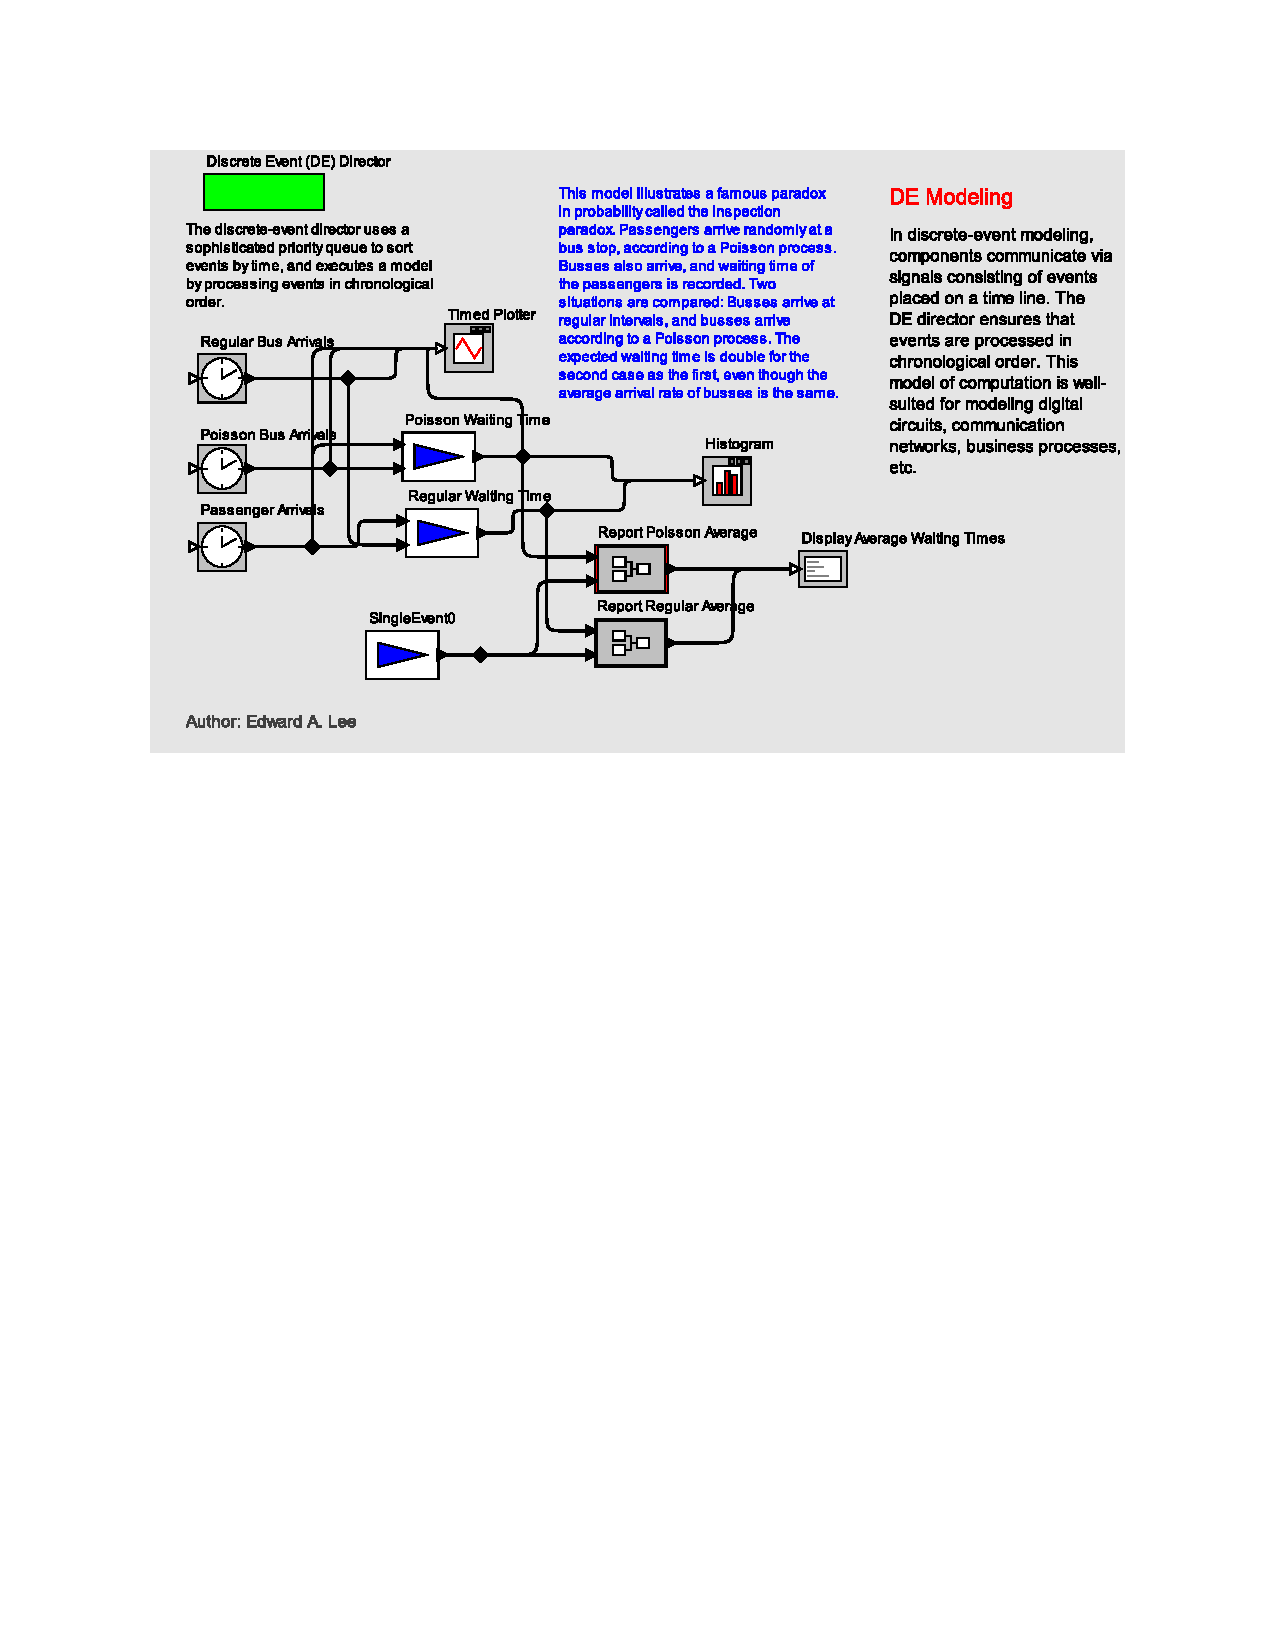
\includegraphics[width=3.5in]{figure.pdf}
  \end{center}

  \caption{\small Figure caption. To get a figure to span two
      columns, use the environment figure* rather than figure.}
  \label{fig-label}
\end{figure}

\section{Using \LaTeX with PDF Figures}

This is a sample document for use with pdflatex, which is
a program that is included with the Miktex distribution
that directly produces PDF files from \LaTeX sources.
To run \LaTeX on this file, you need the following files:
\begin{enumerate}
\item templatePDF.tex (this file)
\item figure.pdf (the figure file)
\item simpleConference.sty (style file)
\item refs.bib (bibiliography file)
\end{enumerate}
\noindent
To create a PDF file, execute the following commands:
\begin{enumerate}
\item pdflatex templatePDF
\item bibtex templatePDF
\item pdflatex templatePDF
\item pdflatex templatePDF
\end{enumerate}
\noindent
Yes (strangely) it is necessary to run pdflatex three times.
The result will be a PDF file (plus several other files that \LaTeX
produces).  You will need a mechanism, of course, for executing
commands on the command line. If you are using Windows, I recommend
installing Cygwin and using its bash shell.

\section{Adam Optimizer}


The Adam Optimizer [1] is a member of a class of "adaptive" gradient descent optimizers which adjust their learning rate $\alpha$ at each iteration in order to converge more efficiently. This adaptive behavior significantly reduces the impact of a badly chosen initial learning rate $\alpha$, which can be difficult to determine. Adam is specifically optimized for sparse datasets as are many similar algorithms in this class. This makes it an excellent candidate for MNIST data which is monochrome and therefore predominantly zero-value. 

The Adam algorithm stores a history of previous gradients $v_t$ and squared gradients $m_t$, also known as first and second moments. In order to compute the current gradient, Adam applies exponentially decaying factors $ \beta_1$ and $\beta_2$ to the first and second moments. It finally calculates bias-adjusted values of these moments $\hat{v}_t , \hat{m}_t $ , and applies a smoothing term $\epsilon$ which avoids division by zero. Pseudocode is given below:

\subsection{Algorithm 1: Adam optimization step}

 while  $ f ( \theta_t ) > \tau $ 

	$ t = t + 1 $

	$g_t = \nabla_{\theta} f_t (\theta_{t-1})$

	$ m_t = \beta \cdot m_{t-1} + (1-\beta_1) \cdot g_t  $

	$ v_t = \beta_2 \cdot v_{t-1} + (1+\beta_2) \cdot g_t^2  $

	$\hat{m}_t =\frac{m_t}{1-\beta_1^t}  $

	$\hat{v}_t = \frac{v_t}{1-\beta_2^t}  $

	
	$ \theta_t = \theta_{t-1} - \alpha \cdot  \frac{{\hat{m}_t}}{\sqrt{\hat{vt}} + \epsilon} $


end while



\section{Performance Characteristics}

The following section compares gradient descent, adam, and BFGS optmizers on a linear least squares Ax = b optimization, and a logistic regression to solve the MNIST problem.

\subsection{Gradient Descent}


    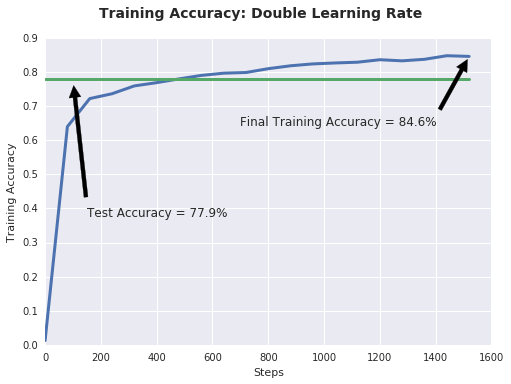
\includegraphics[width=3.5in]{plot1-GradDescent.png}



Suppose you wish to include a figure, like that in figure \ref{fig-label}.
The simplest mechanism is to install Adobe Acrobat, which includes
a ``printer'' called ``Acrobat Distiller.'' Printing to this printer
creates a PDF file, which can be included in a document as shown
here.  To include Ptolemy II models \cite{PtolemyVol1:04},
just print to the distiller from within Vergil and reference
the PDF file in your \LaTeX document.

There is a bit more work to do, however.
The file that is produced by the distiller represents
a complete page, not the individual figure.
You can open it in using Acrobat (version 5.0 or later),
and select Document $\rightarrow$ Crop Pages from the menu.
In the resulting dialog, check ``Remove White Margins.''
Save the modified PDF file in a file and then reference
it in the \LaTeX file as shown in this example.

An alternative is to generate EPS (encapsulated postscript),
but the process is much more complex and fragile.
I recommend using pdflatex and Adobe Acrobat.

\bibliographystyle{abbrv}
\bibliography{refs}
\end{document}
